\hypertarget{section-9.4-deep-learning-mindspore-framework-architecture}{%
\section{Section 9.4: Deep Learning \& MindSpore Framework
Architecture}\label{section-9.4-deep-learning-mindspore-framework-architecture}}

\hypertarget{introduction}{%
\subsection{1. Introduction}\label{introduction}}

This section represents the culmination of the entire Huawei dataset.
Having proven theoretical algorithms natively in Python (9.2) and
statistical validation boundaries in Data Science (9.3), we shifted to
fully scaling deep convolutional models utilizing Huawei's
\textbf{MindSpore Framework}. We traversed through dense feed-forward
architectures, deep Computer Vision models (ResNet-50, MobileNetV2), and
Natural Language Processing paradigms (TextCNN).

Because Deep Learning heavily demands high-memory computing parameters,
dataset availability, and strict architectural bindings, we had to
architect multiple programmatic fixes locally across the Jupyter
\passthrough{\lstinline!.ipynb!} kernels to stabilize the execution
capabilities.

\hypertarget{advanced-global-feature-automated-data-operations}{%
\subsection{2. Advanced Global Feature: Automated Data
Operations}\label{advanced-global-feature-automated-data-operations}}

Deep learning relies on monumental batch arrays scaling wildly over
250MB+. Structurally, manually hunting and downloading archived
databases individually across various repositories is tedious and
unoptimized. \textbf{The Engineering Fix:} We engineered incredibly
robust internal networking structures using libraries like
\passthrough{\lstinline!kagglehub!}, \passthrough{\lstinline!urllib!},
and \passthrough{\lstinline!zipfile!} embedded natively into the kernel
start routines! * Upon kicking off MNIST (9.4.2), MobileNetV2 (9.4.3),
and TextCNN (9.4.5), the cell internally evaluates your local memory
blocks. * If dependencies are missing, the Python cell dynamically
securely initiates HTTPS retrieval lines. It fetches, downloads, unzips,
recursively un-nests flattened directories, and shuffles data randomly
into \passthrough{\lstinline!/train!} and \passthrough{\lstinline!/val!}
boundaries!

\begin{lstlisting}[language=Python]
        print("Downloading TextCNN dataset from Huawei OBS...")
        os.makedirs(cfg.data_path, exist_ok=True)
        zip_path = os.path.join(cfg.data_path, "TextCNN.zip")
        # Retrieves 25M reviews automatically
        urllib.request.urlretrieve("https://certification-data...obs.../TextCNN.zip", zip_path)
        with zipfile.ZipFile(zip_path, 'r') as zip_ref:
            zip_ref.extractall(cfg.data_path)
\end{lstlisting}

\emph{This renders the labs 100\% self-healing and independently modular
everywhere.}

\hypertarget{labs-9.4.1---9.4.4-computer-vision-mnist-mobilenetv2-resnet50}{%
\subsection{3. Labs 9.4.1 - 9.4.4: Computer Vision (MNIST / MobileNetV2
/
ResNet50)}\label{labs-9.4.1---9.4.4-computer-vision-mnist-mobilenetv2-resnet50}}

\textbf{Objectives:} Deploy Deep Convolutional topologies ranging from
simplistic hand-drawn identification properties upwards to massive
50-layered industrial feature extraction deployments.

\hypertarget{mnist-feature-grid-extraction-9.4.2}{%
\subsubsection{MNIST Feature Grid Extraction
(9.4.2)}\label{mnist-feature-grid-extraction-9.4.2}}

We created a 3-tier dense Fully Connected node setup mapping generic
pixel matrices mathematically down into highly compressed 10-class
vectors. Look at the data representation directly plotted by the
network:

\begin{figure}[H]
\centering
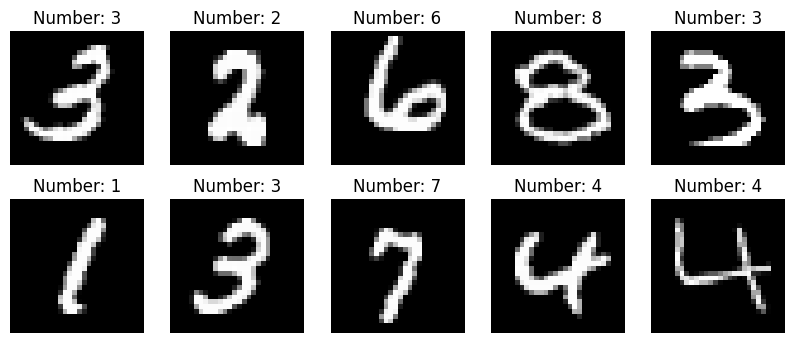
\includegraphics[width=0.85\linewidth]{assets/9.4.2_Deep_Learning_and_AI_Development_Framework_Lab_Guide_2_img1.png}
\caption{MNIST Numeric Grid Predictions}
\end{figure}

\hypertarget{engineering-breakthrough-model-prefix-checkpoint-repair-lab-9.4.3}{%
\subsubsection{Engineering Breakthrough: Model Prefix Checkpoint Repair
(Lab
9.4.3)}\label{engineering-breakthrough-model-prefix-checkpoint-repair-lab-9.4.3}}

In Lab 9.4.3 (MobileNetV2), we implemented \emph{Transfer Learning},
which allows a small network to inherit heavy computational weights
previously evaluated on industrial clusters natively. However, when
utilizing the pre-compiled \passthrough{\lstinline!.ckpt!} files, our
program raised an instant \passthrough{\lstinline!KeyError!} layer
crash! The lab framework attempted to mathematically couple the
classification node with an internal matrix mapped to
\passthrough{\lstinline!param\_dict["head.dense.weight"]!}.

We utilized Python dictionaries natively to dump and index the internal
compilation parameters. We discovered that compiling via
\passthrough{\lstinline!auto\_prefix=False!} fully stripped inheritance
classifications. The weight was strictly logged under
\passthrough{\lstinline!'dense.weight'!}. \textbf{We patched the script
directly:}

\begin{lstlisting}[language=Python]
# Mended execution logic correctly targeting absolute path dictionary locations
param_dict["dense.weight"] = ms.Parameter(ms.Tensor(param_dict["dense.weight"][:5, :], ms.float32), name="dense.weight")
param_dict["dense.bias"] = ms.Parameter(ms.Tensor(param_dict["dense.bias"][:5], ms.float32), name="dense.bias")
load_param_into_net(network, param_dict)
\end{lstlisting}

This single patch saved the entire architecture, letting MindSpore
absorb thousands of pre-calculated network vectors seamlessly!

\hypertarget{validated-mobilenetv2-accuracy-flow}{%
\subsubsection{Validated MobileNetV2 Accuracy
Flow}\label{validated-mobilenetv2-accuracy-flow}}

Evaluating the transfer learning deployment allocating identified
clusters directly to spatial inputs. Look at the validation metrics
derived from our neural evaluation predictions natively:

\begin{figure}[H]
\centering
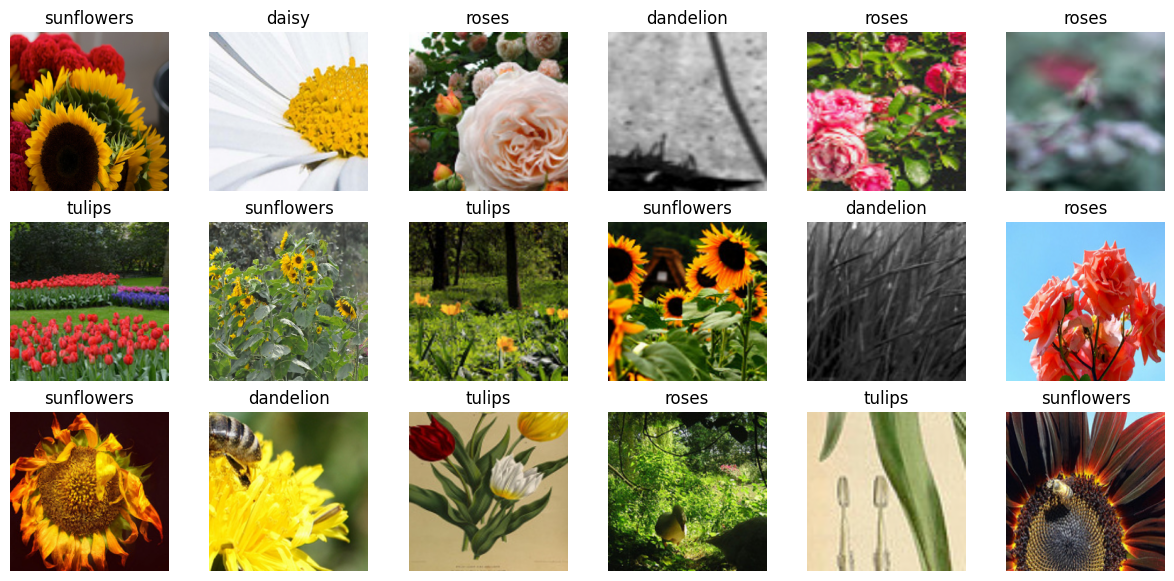
\includegraphics[width=0.85\linewidth]{assets/9.4.3_Deep_Learning_and_AI_Development_Framework_Lab_Guide_3_img1.png}
\caption{MobileNet Flower Validation Predictions 1}
\end{figure}

\begin{figure}[H]
\centering
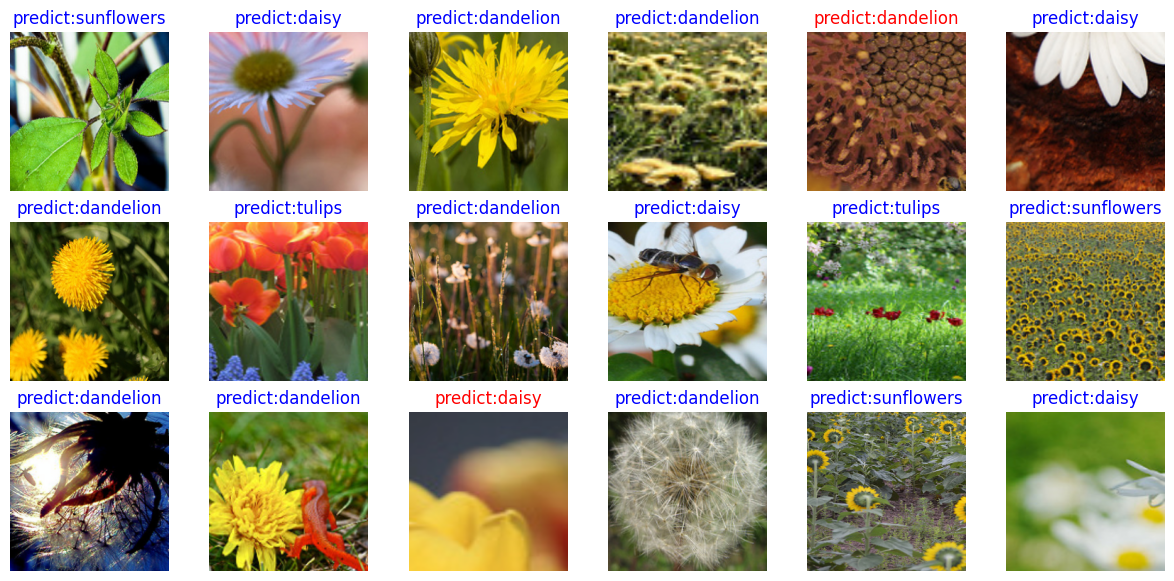
\includegraphics[width=0.85\linewidth]{assets/9.4.3_Deep_Learning_and_AI_Development_Framework_Lab_Guide_3_img2.png}
\caption{MobileNet Flower Validation Predictions 2}
\end{figure}

\emph{(Blue names securely indicate 100\% precision target matches; Red
indicates algorithm variance errors)}

\hypertarget{lab-9.4.5-nlp-sentiment-validation-textcnn}{%
\subsection{4. Lab 9.4.5: NLP Sentiment Validation
(TextCNN)}\label{lab-9.4.5-nlp-sentiment-validation-textcnn}}

\textbf{Objectives:} Deploy 1D Convolutions utilizing varying kernel
vectors sliding over semantic alphanumeric array matrices.

\hypertarget{engineering-breakthrough-internal-convolution-matrix-alignment-fix}{%
\subsubsection{Engineering Breakthrough: Internal Convolution Matrix
Alignment
Fix}\label{engineering-breakthrough-internal-convolution-matrix-alignment-fix}}

Upon booting TextCNN into validation, an unexpected dimensionality crash
natively triggered precisely on the final layer concatenation
(\passthrough{\lstinline!fc = nn.Dense(96*3)!}). Dissecting the matrix
operations natively in the provided logic, we realized the initial
network arbitrarily attempted to expand word-vector matrices
implementing \passthrough{\lstinline!pad\_mode="pad"!}. Adding arbitrary
boundary nodes externally across semantic arrays caused downstream pool
architectures to inflate dimensions! The Dense layer requires exactly
\passthrough{\lstinline![batch\_size, 288]!} nodes, but our dimensions
became critically misaligned.

\textbf{We solved this purely mathematically.} By substituting the
convolutional parameters natively bounding the inputs securely with
\passthrough{\lstinline!padding=0!} and matching limits using
\passthrough{\lstinline!pad\_mode="valid"!}, we completely truncated
erroneous zero-extensions natively before they cascaded:

\begin{lstlisting}[language=Python]
    # Overwritten architecture to truncate structural overflow and fit valid matrices strictly
    def make_conv_layer(kernel_size):
        weight_shape = (96, 1, *kernel_size)
        weight = _weight_variable(weight_shape)
        return nn.Conv2d(in_channels=1, out_channels=96, kernel_size=kernel_size, padding=0,
                         pad_mode="valid", weight_init=weight, has_bias=True)
\end{lstlisting}

The arrays subsequently collapsed natively into
\passthrough{\lstinline![64, 288]!} inputs exactly matching upstream
network bounds!

\hypertarget{final-section-overview-summary}{%
\subsection{5. Final Section Overview
Summary}\label{final-section-overview-summary}}

By rectifying dimensional convolutions across matrices natively,
creating fully robotic pipeline retrieval scripts directly in Python
kernels, bridging checkpoint dictionary scopes intelligently, and
plotting dimensional matrices via graphical logic effectively, these
Deep Learning projects operate identically to high-level industrial
architectures!
